\section*{2.2 The Formula}
Let $G=(V,E)$ be a graph. For every $e\in E(G)$ we introduce a variable $x_e$. Given a charge $c:V\to\{0,1\}$, the Tseitin formula on $G$ with charge $c$ is the Boolean formula
\begin{equation}
\operatorname{Tseitin}(G,c):=\bigwedge_{u\in V(G)}
\left(\sum_{e\in E(G):u\in e}x_e\equiv c(u)\pmod2\right).\tag{1}
\end{equation}
If $G$ has maximum degree $k$ then this can be expressed as a $k$-CNF formula on $m=|E(G)|$ variables and $|V(G)|2^{k-1}$ clauses. Usually in proof complexity, the charge $c$ is chosen so that $\operatorname{Tseitin}(G,c)$ is unsatisfiable. In this paper, all charges will be0, and $\operatorname{Tseitin}(G,0)$ is obviously satisfiable: set all variables to0. We will hence drop $c$ from the notation and simply write $\operatorname{Tseitin}(G)$ to denote this formula. The constraint $\sum_{e\in E(G):u\in e}x_e\equiv0\pmod2$ is called the Tseitin constraint of vertex $u$. Given a set $B$ of pairs of edges in $G$ consider the following formula
\[
\operatorname{Tseitin}(G)\wedge\bigwedge_{\{e,f\}\in B}(\bar x_e\vee\bar x_f).
\]
The constraint $(\bar x_e\vee\bar x_f)$ is called a bridge constraint. It is easy to see that $\mathbf0$ is the unique satisfying assignment of this formula if and only if every cycle in $G$ contains a bridge in $B$. We will consider a particular instantiation of bridges given by graph homomorphisms. A graph homomorphism from a graph $G$ to a graph $H$ is a function $\phi:V(G)\to V(H)$ such that $\{\phi(u),\phi(v)\}\in E(H)$ whenever $\{u,v\}\in E(G)$. Thus, $\phi$ also induces a function from $E(G)$ to $E(H)$; $\phi(\{u,v\}):=\{\phi(u),\phi(v)\}$. Given $G,H$, and a homomorphism $\phi$ from $G$ to $H$, we define a Tseitin formula with bridges on the variable set $\{x_e\mid e\in E(G)\}$:
\begin{equation}
\operatorname{TseitinBridge}(G,H,\phi):=
\operatorname{Tseitin}(G)\wedge
\bigwedge_{\substack{e,f\in E(G)\\e\ne f,\phi(e)=\phi(f)}}(\bar x_e\vee\bar x_f).\tag{2}
\end{equation}
For brevity, we write $V=V(G)$ and $E=E(G)$.
\begin{authorclaim}{Observation 5}
If $\operatorname{girth}(G)>|E(H)|$ then $\operatorname{TseitinBridge}(G,H,\phi)$ is uniquely satisfiable by $\mathbf0$.
\end{authorclaim}
\begin{proof}
Let $\alpha\ne\mathbf0$ be a total assignment. Let $F:=\{e\in E(G)\mid\alpha(x_e)=1\}$. If some vertex $u$ has degree1 in $(V,F)$, then $\alpha$ violates its Tseitin constraint. Otherwise, $(V,F)$ has a cycle, which has length at least $\operatorname{girth}(G)$. By the pigeonhole principle, this cycle contains two edges $e,f$ such that $\phi(e)=\phi(f)$, and thus $\alpha$ violates their bridge constraint.
\end{proof}
\paragraph{Locally Injective Homomorphisms}
A homomorphism $\phi$ is called locally injective if for every $u\in V(G)$ and any two of its neighbors $v_1$ and $v_2$, it holds that $\phi(v_1)\ne\phi(v_2)$. Note that $\phi:G\to H$ being locally injective immediately implies that $\deg_G(u)\le\deg_H(\phi(u))$. We call $\phi$ locally bijective if, additionally, $\deg_G(u)=\deg_H(\phi(u))$ for all vertices $u$ of $G$. Note that a locally bijective homomorphism bijectively maps the neighborhood of $u$ to the neighborhood of $\phi(u)$. The graph $G$ is called a covering graph of $H$ or a lift of $H$.
\begin{center}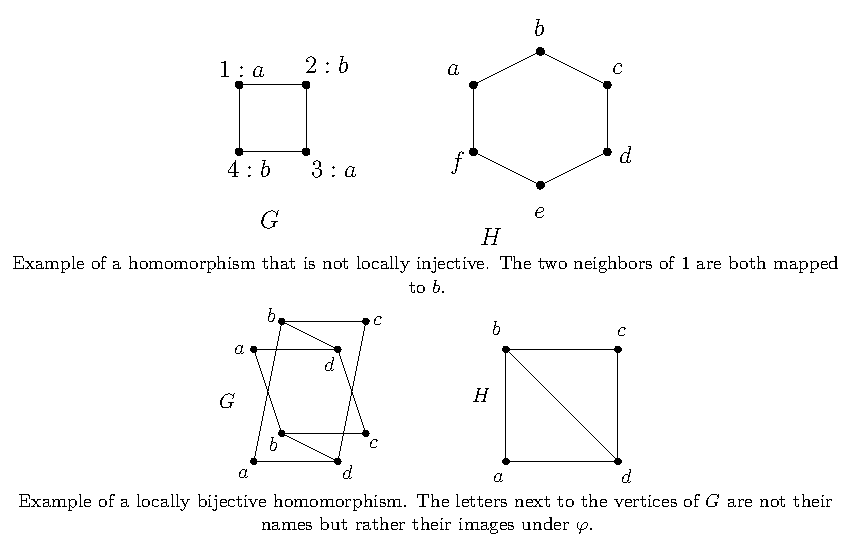
\includegraphics[width=.95\linewidth]{homomorphism-examples.pdf}\end{center}
\begin{authorclaim}{Theorem 6}
Let $G$ be a graph on $n$ vertices and $m$ edges. Suppose there is a locally injective graph homomorphism $\phi:G\to H$ for some graph $H$ with $|E(H)|<\operatorname{girth}(G)$. Then for all $\epsilon>0$ and $w:=\sqrt{\epsilon\cdot\operatorname{girth}(H)/2}-3$, the success probability of PPSZ with heuristic $R_w$ on $\Phi:=\operatorname{TseitinBridge}(G,H,\phi)$ is at most
\[
\Pr[\operatorname{ppsz}(\Phi,R_w)]\le2^{-m+(1+\epsilon)n}.
\]
\end{authorclaim}
\begin{proof}[Proof of Theorem2 using Theorem6]
We first show how to construct $F_m$ for infinitely many $m$. Let $n_0$ be some given, sufficiently large even integer. A well-known fact, first proven by Erd\H{o}s and Sachs [4], is that there is a $k$-regular graph $G_0$ on $n_0$ vertices having girth at least $g_0:=\log n_0/\log(k-1)$. Set $n_1:=\lfloor2(g_0-1)/k\rfloor$ or $n_1:=\lfloor2(g_0-1)/k\rfloor-1$, whichever is even, and let $G_1$ be a $k$-regular graph on $n_1$ vertices, such that $\operatorname{girth}(G_1)\ge g_1:=\log n_1/\log(k-1)$. This exists, provided that $n_0$ is sufficiently large. Note that $G_1$ has at most $g_0-1<\operatorname{girth}(G_0)$ edges.
A result by Angluin and Gardiner [1] states that there is a common lift $G$ of $G_0$ and $G_1$. That is, $G$ is a covering graph of $G_0$ and of $G_1$. Being a lift of a $k$-regular graph, $G$ is $k$-regular as well. A closer inspection of their proof reveals that $n:=|V(G)|\le4n_0n_1$.
Let $m:=kn/2$ be the number of edges in $G$. We set $\Phi_m:=\operatorname{TseitinBridge}(G,G_1,\phi_1)$, where $\phi_1$ is the locally bijective homomorphism from $G$ to $G_1$.
It is not difficult to see that lifting cannot decrease the girth, and thus $\operatorname{girth}(G)\ge\operatorname{girth}(G_0)>|E(G_1)|$. Thus, we can apply Theorem6 to $G,G_1$, and $\phi_1$, and conclude that the success probability of PPSZ on $\Phi_m$ is at most $2^{-m+(1+\epsilon)n}$ when using heuristic $R_w$. A quick calculation shows that $g_1\ge\log\log m/\log k$ if $n_0$ is sufficiently large, and thus
\[
w\ge\sqrt{\epsilon\cdot\frac{\log\log m}{2\log k}}-3.
\]
This construction gives us an infinite set $M\subseteq\mathbb N$ and, for each $m\in M$, a satisfiable $k$-CNF formula $F_m$ on $m$ variables for which the claimed hardness result holds. By a simple tweaking of the construction, we can ensure that $M$ is "reasonably dense", meaning that there is some $m^*\in M\cap[m-\log m,m]$ for all sufficiently large $m$. We then let $F_{m^*}$ be $F_m$, plus $m-m^*$ dummy variables. The success probability is then at most $2^{-m^*(1-2(1+\epsilon)/k)}\le\operatorname{poly}(m)2^{-m(1-2(1+\epsilon)/k)}$. We leave the details to the reader.
\end{proof}
